\section{Geometry}
\subsection{The triangle primitive}
This section focuses on the basic math of ray tracing. In a ray tracer so called primary rays are shot from a camera
onto a scene. Irreducible objects or geometric primitives are defined. These make up a scene. In order to compute an
image from this given scene, the ray-object intersection point closest to the camera has to be found. 
Various primitives have been implemented the most important one is the triangle. As triangle meshes can be used, to
approximate more complex shapes. A triangle is defined by the three points $\mathbf{a},\mathbf{b},\mathbf{c}$, that make up its edges. If the edges are ordered counterclockwise the triagle normal can be computed using the formula:
\footnote{This section in based on Ray Tracing from the gound up page 362 and onward.}
\begin{equation}
\mathbf{n} = (\mathbf{b} - \mathbf{a}) \times (\mathbf{c} - \mathbf{a}) /
 \|( \mathbf{b} - \mathbf{a} ) \times ((\mathbf{c} - \mathbf{a})\|.
\label{eq:triNormal}
\end{equation}
To find triangle intersection points barycentric coordinates ($\alpha, \beta, \gamma$) are used. These coordinates allow to describe any point in the plane of the triangle as:
\begin{align}
\mathbf{p}(\alpha,\beta,\gamma) = \alpha \mathbf{a} + \beta \mathbf{b} + \gamma \mathbf{c}, \\
\text{with } \alpha + \beta + \gamma = 1.
\end{align}
If $\mathbf{p}$ is inside of the plane the inequalities,
\begin{align}
0 < \alpha < 1,
0 < \beta < 1,
0 < \gamma < 1,
\label{ineq:inCond}
\end{align}
are satisfied. By substituting $\alpha = 1 - \beta - \gamma$ into the equation and setting $\mathbf{p} = \mathbf{r}(t)$ with $\mathbf{r} = \mathbf{o} + t \cdot \mathbf{d}$ for a ray the following equation is obtained:
\begin{align}
\mathbf{o} + t\mathbf{d} = \mathbf{a} + \beta(\mathbf{b} - \mathbf{a}) + \gamma (\mathbf{c} - \mathbf{a}).
\end{align}
Which can be brought into the form $\mathbf{A}\mathbf{x} = \mathbf{b}$ with $\mathbf{x} = \begin{pmatrix}
\beta & \gamma & t \\
\end{pmatrix}^T$:
\begin{align}
\begin{pmatrix}
a_x - b_x & a_x - c_x & d_x \\
a_y - b_y & a_y - c_y & d_y \\
a_z - b_z & a_z - c_x & d_z \\
\end{pmatrix}
\begin{pmatrix}
\beta \\ \gamma \\ t \\
\end{pmatrix}
= 
\begin{pmatrix}
a_x - o_x \\
a_y - o_y \\
a_z - o_z \\
\end{pmatrix}.
\label{eq:triInt}
\end{align}
Equation~\ref{eq:triInt} could in principle be given to a linear algebra subroutine for solution. If the inequalities~\ref{ineq:inCond} are satisfied and $t > \epsilon$. Where epsilon is a small positive number used to prevent self intersection. A valid intersection has been found. However this
is not the most efficient way to proceed. Always solving the whole equation system is not necessary all the time.
Using Cramers rule the a set of equations can be derived and the intersection method can return as soon as one 
condition is violated. This way unnecessary computations can be avoided. \footnote{See Ray Tracing from the Ground up page 366 for further details.}

\subsection{The plane primitive}
Another important primitive is the plane. These objects can be defined by a normal $\mathbf{n}$ which determines the orientation of the plane and $\mathbf{a}$ which determines where it is.\footnote{Ray Tracing from the ground up page 31.} 
For a point $\mathbf{p}$ on the plane, the condition 
\begin{equation}
(\mathbf{p} - \mathbf{a})^T  \mathbf{n} = 0
\label{eq:plane}
\end{equation} 
must hold. This is the same as asking for the cosine of the angle between the vector on the plane and normal to be zero. Or equivalently saying that the vectors $(\mathbf{p} - \mathbf{a})$ and $\mathbf{n}$ must form a $90^{\circ}$ angle. To check if a given ray intersects a plane the ray must be plugged into equation~\ref{eq:plane} which yields:\footnote{Ray Tracing from the Ground up page 54.}
\begin{equation}
(\mathbf{o} + t\mathbf{d} - a)^T \mathbf{n} = 0.
\end{equation}
Solving for $t$ then leads to:
\begin{equation}
t = (\mathbf{a}^T\mathbf{n} -  \mathbf{o}^T\mathbf{n}) ) / (\mathbf{d}^T \mathbf{n}).
\end{equation}
If then $ t > \epsilon$ a valid intersection was computed. The exact location of the hit point can be found from the ray equation $\mathbf{p}(t) = \mathbf{o} + t\mathbf{d}$. 

\subsubsection{The rectangle primitive}
A rectangle is simply a subset of all the points contained in a plane therefore the same equations can be used. Additionally the conditions
\begin{align}
\|p_x\| < 1.0,
\|p_y\| < 1.0,
\end{align}
have to be enforced to turn a the $x$,$y$-plane into a rectangle around the origin. This unit plane can later be rotated and scaled using transformations to fit into a desired scene.

\subsubsection{The circle primitive}
A circle in the $x$,$y$ plane is obtained by a procedure analogue to the one which lead to rectangles if instead the condition
\begin{align}
\sqrt{p_x^2 + p_y^2} < 1.0
\end{align}
is used. This circle can similarly be transformed to fit into any scene. 

\subsection{The sphere primitive}
A sphere is a set of points located within a given distance r around a specified point $\mathbf{c}$. For any point $\mathbf{p}$ within this sphere the condition:
\begin{align}
\|\mathbf{p} - \mathbf{c} \| &\leq r \\
\text{or } (\mathbf{p} - \mathbf{c})^T (\mathbf{p} - \mathbf{c}) &\leq r^2
\end{align}
must hold. For a sphere around the origin with radius one $\mathbf{c} = 0$, $r^2 = 1$ and substituting $\mathbf{p} = \mathbf{o} + t\mathbf{d}$ the expression below is obtained:
\begin{align}
(\mathbf{o} + t\mathbf{d})^T (\mathbf{o} + t\mathbf{d}) - 1 = 0 
\end{align}
Now using an equality instead of an inequality to compute the intersection with the outer bound of the sphere. 
The distributive property of the dot product leads to:
\begin{align}
t^2 \mathbf{d}^T \mathbf{d} + 2t\mathbf{o}^T \mathbf{d} + \mathbf{o}^T \mathbf{o} - 1 = 0.
\end{align}
The obtained quadratic equation can be solved using standard methods with:
\begin{align}
a = \mathbf{d}^T \mathbf{d} \\
b = 2\mathbf{d}^T \mathbf{o} \\
c = \mathbf{o}^T \mathbf{o} - 1 \\
\text{then  } t = \frac{-b \pm \sqrt{b^2 - 4ac}}{2a}
\end{align}
It is possible for learn the number of intersections from the discriminant $d = b^2 - 4ac$. If $d < 0$ there will be no intersections, one if $d = 0$ and two if $d > 0$. If two intersections are found the one with the smaller t should be used, as it will be closer to the camera.\footnote{Ray Tracing from the Ground up page 57}

\section{Object Transformations}
In order to move, rotate or scale the objects defined earlier four dimensional transformation matrices are defined. Four dimensions are used, as three dimensional translations can be expressed as a matrix operation. \\ 
Scaling can be done by using\footnote{Ray Tracing from the ground up page 404}:
\begin{align}
T_{scale} = \begin{pmatrix}
a &   &   &\\
  & b &   &\\
  &   & c &\\
  &   &   & 1 \\
\end{pmatrix}
\;\;\;\; T_{scale}^{-1} = 
\begin{pmatrix}
1/a &   & & \\
  & 1/b & & \\
  &   & 1/c & \\
  &   &     & 1 \\
\end{pmatrix}
\end{align}
Translation is working with:
\begin{align}
T_{translate} = \begin{pmatrix}
1 &   &  & d_x\\
  & 1 &  & d_y\\
  &   & 1 & d_z \\
  &   &   & 1 \\
\end{pmatrix}
\;\;\;\; T_{translate}^{-1} = 
\begin{pmatrix}
1 &   &  & -d_x\\
  & 1 &  & -d_y\\
  &   & 1 & -d_z \\
  &   &   & 1 \\\end{pmatrix}
\end{align}
Rotation around the tree axes:
\begin{align}
T_x = \begin{pmatrix}
	1&		&		&		&				\\
	&		\cos(\theta)&	-\sin(\theta)&	\\
    &		\sin(\theta)&	\cos(\theta)	&	\\
	&		&		&		1				
\end{pmatrix} \\
T_y = \begin{pmatrix}
\cos(\theta) &	    &		\sin(\theta) &	 &	\\
	         &	   1&	                &	 &	\\
-\sin(\theta) &	    &		\cos(\theta) &	& 	\\
		     &	    &		            &		1 \\\end{pmatrix} \\
T_z = \begin{pmatrix}
\cos(\theta)&	-\sin(\theta)&  & &	 &	\\
\sin(\theta)&	\cos(\theta)&&	                &	 &	\\
            &    &		1 &	& 	\\
		     &	    &		            &		1 \\
\end{pmatrix} \\
\end{align}
The inverse rotations can be obtained by using $-\theta$ in place of $\theta$ or by transposing the matrices. Several
transformations can be combined by matrix multiplication. \\
Instead of transforming objects it is common practice in ray tracing to transform rays. Prior to intersection testing
a ray ($\mathbf{r}(t) = \mathbf{o} + t\mathbf{d}$) is multiplied with the inverse transformation matrix. The obtained transformed ray is then intersected with the unchanged object. The hit point is found and transformed back into the
original space using the transformation matrix. \footnote{Ray Tracing from the Ground up page 418.} 
For normals the process is slightly more complicated. \footnote{ Fundamentals of
Computer Graphics, Lecture 3 Transformations, Philip Dutr\'e,  slide 60}
In the unchanged space the normal must be orthogonal to infinitely small vectors along the surface $\mathbf{n}^T \mathbf{m} = 0$. The same must be true for the transformed space $\mathbf{n'}^T\mathbf{m'} = 0$. Like points differences between points will be transformed by the original transformation matrix $\mathbf{Tm} = \mathbf{m}'$. Furthermore a matrix multiplied with its inverse is the identity $\mathbf{T}^{-1}\mathbf{T} = \mathbf{I}$. This leads to the derivation:
\begin{align}
\mathbf{n}^T\mathbf{m} = 0 \\
\mathbf{n}^T\mathbf{I}\mathbf{m} = 0 \\
\mathbf{n}^T\mathbf{T}^{-1}\mathbf{T}\mathbf{m} = 0 \\
(\mathbf{n}^T\mathbf{T}^{-1})(\mathbf{T}\mathbf{m}) = \mathbf{n'}^T\mathbf{m'} =  0 \\
(\mathbf{n}^T\mathbf{T}^{-1})(\mathbf{T}\mathbf{m}) = \mathbf{n'}^T(\mathbf{Tm}) \\
\mathbf{n}^T\mathbf{T}^{-1} = \mathbf{n'}^T \\
\Rightarrow \mathbf{n'} = \mathbf{T}^{-T}\mathbf{n}
\end{align}
Thus normals will be transformed by the transposed inverse transformation matrix.

\section{Point Lights}
Point lights emit light from a single point only. To create a point light its location $\mathbf{p}_l$, color $\mathbf{c}_l$ and intensity $l_s$ have to be stored. 


\section{Shading}
Shading with respect to point lights can be done with a simplified form of the rendering equation. Taking only into account ambient and distance attenuated direct illumination one arrives at:\footnote{Ray tracing from the ground up page 265. } \footnote{Computergrafiek Project sessie 1 page 41. }
\begin{equation}
L(\mathbf{p},\mathbf{\omega}) = \rho_a \mathbf{c}_d \cdot (l_s \mathbf{c}_l) + \sum_{j=1}^{n}(\rho_d \mathbf{c}_d/ \pi)
\cdot (l_{s,j}\mathbf{c}_{l,j})(\mathbf{n}^T\mathbf{l}_j)/(d_j^2) \cdot V(\mathbf{p},\mathbf{p}_{l,j})
\end{equation} 
With $\rho$ describing the material reflectivity with respect to ambient or diffuse illumination. Light intensity is denoted by $l$. The $\mathbf{c}$ vectors represent r,g,b color values, $\mathbf{n}$ denotes the normal vector. The vector $\mathbf{\omega}$ points from $\mathbf{p}$ to the camera and $\mathbf{l}$ to the light source. Finally the visibility function $V$ is one if the location of the point light $\mathbf{p}_l$ is visible from the object intersection point $\mathbf{p}$ and zero if not.


\section{Camera}
In this project a perspective camera is used. To set it up the resolution ($r_x,r_y$), origin $\mathbf{e}$, view direction $\mathbf{l}$ , spacial orientation $\mathbf{up}$ and the field of view angle $\delta$ have to be provided. Using $\delta$ and the resolution data the width $w$ and hight $h$ of the view plane can be computed:
\begin{align}
w = 2 \cdot d \tan(\delta/2) \\
h = r_y \cdot w \cdot 1/r_x
\end{align}
The view plane distance can be kept at $d = 1$ for all practical purposes. Changing $d$ would change the zoom of the camera just like changing the view angle does. Making $d$ a variable user parameter would therefore have no additional value. 
In order to describe the view plane and generate primary rays more easily the camera coordinate system is used. This system is set up using:
\begin{align}
\mathbf{w} &= (-1) \cdot \mathbf{l} \\
\mathbf{u} &= (\mathbf{up} \times \mathbf{w})/ \|\mathbf{up} \times \mathbf{w} \| \\
\mathbf{v} &= \mathbf{w} \times \mathbf{u}
\end{align}
In this coordinate system points on the view plane can be expressed in terms of $\mathbf{u}$ and $\mathbf{v}$, which in turn become primary ray directions if $\mathbf{w}$ is subtracted. With the known camera position as the ray origin all necessary information to generate primary rays is available.

\section{Python or Java}
In this section two basic ray tracing implementations using only diffuse shading without shadows in Java and Python will be compared. A scene consisting of a plane with a chess like procedural texture as well a two spheres will be set up in both languages. 
\begin{figure}
\centering
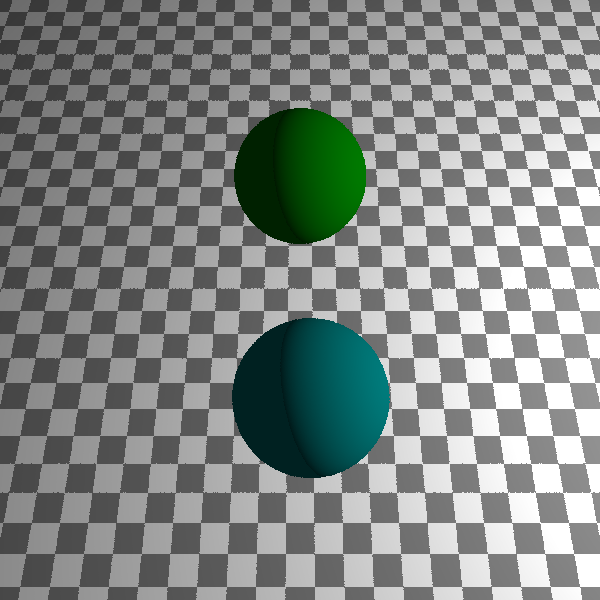
\includegraphics[width=0.35\linewidth]{./img/javaSphere2}
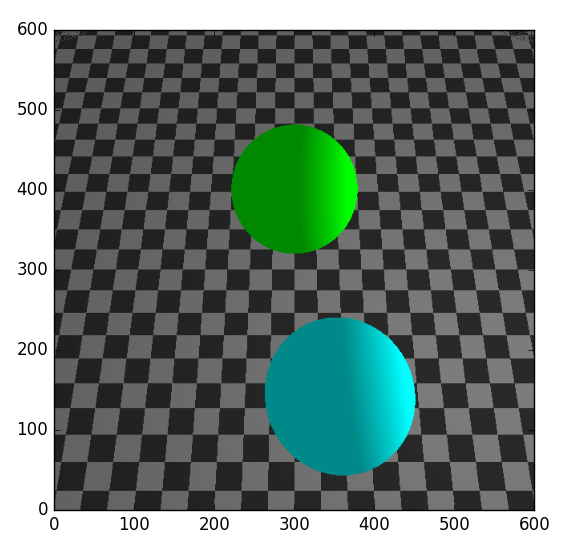
\includegraphics[width=0.40\linewidth]{./img/spherePython}
\caption{Two similar scenes rendered using comparable rendering code in Java and Python .}
\label{fig:spherePython}
\end{figure}
The rendered 600x600 pixel images are shown in figure~\ref{fig:spherePython}. With the result of the java code on the left and the python version on the right. The first image took 1.18s  to compute while the second was ready after 16.61s. The python code is executed faster if it is run a second time as compiled python files will be generated, but for this scene it never falls under 10s. A popular method to speed up python code is to use the typed Cython dialect.\footnote{Cython: The Best of Both Worlds,Computing in Science \& Engineering, S. Behnel; R. Bradshaw et al., Computing in Science \& Engineering \url{http://ieeexplore.ieee.org/stamp/stamp.jsp?tp=&arnumber=5582062}} However cythons multi-threaded capabilities are limited due to pythons global interpreter lock, additionally cython compiled classes can only be accessed from compiled code, which leads to a significant extra amount of code conversion work. Therefore the remainder of the project was done exclusively in Java. Javas strong typing avoids the python overhead which slowed down the ray tracing process considerably, as the python interpreter looses a lot of time determining the type of every object. 
